As a consistency check we have performed a closure test verifying that after
applying two opposite \ekos{} to a custom initial condition
we are able to recover the initial \pdf{}. Specifically, the product of the
two kernels is an identity both in flavor and momentum space up to
the numerical precision. The results are shown in \cref{fig:closure_test} in case of \nnlo{} evolution
crossing the bottom threshold scale $\mu_{F}=m_{b}$. The differences between
the two inversion methods are more visible for singlet-like quantities,
because of the non-commutativity of the matching matrix $\tilde{\mathbf{A}}_{S}^{(n_f)}$.  

\begin{figure}
    \begin{center}
    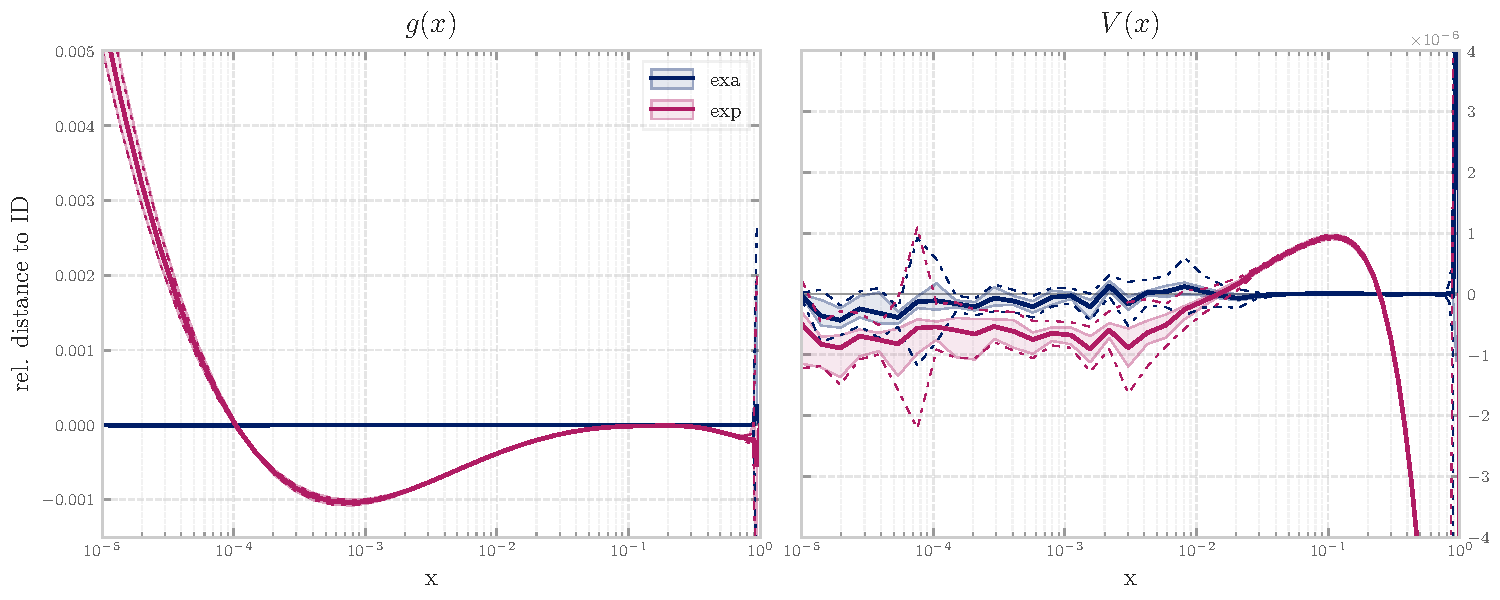
\includegraphics[width=\textwidth]{ch-eko/closure_test.pdf}
    \end{center}
    \caption{Relative distance of the product of two opposite \nnlo{} \ekos{}
        and the identity matrix, in case of exact inverse and expanded
        matching (see \cref{eq:eko/invmatchingexp}) when crossing the bottom
        threshold scale $\mu_{b}^2=\SI[parse-numbers=false]{4.92^2}{\GeV^2}$. In particular the lower scale is chosen $\muF^2=\SI[parse-numbers=false]{4.90^2}{\GeV^2}$, 
        while the upper is equal to $\muF^2=\SI[parse-numbers=false]{4.94^2}{\GeV^2}$, 
        \label{fig:closure_test}
    }
\end{figure}

Special attention must be given to the heavy quark distributions which are
always treated as intrinsic, when performing backward evolution.
In fact, if the initial \pdf{} (above the mass threshold) contains an intrinsic contribution, this has to be evolved
below the threshold otherwise momentum sum rules can be violated.
This intrinsic component is then scale independent and fully decoupled
from the evolving (light) \pdfs.
On the other hand, if the initial \pdf{} is purely perturbative, it vanishes
naturally below the mass threshold scale after having applied the
inverse matching.
In this context, \eko{} has been used in a recent study to determine, for the first time,
the intrinsic charm content of the proton~\cite{Ball:2022qks}.
